\documentclass[11pt]{article}
\usepackage{amsmath}
\usepackage{amssymb}
\usepackage{graphicx}
\usepackage{geometry}[0.9in]
\usepackage{url}
\usepackage{physics}

\renewcommand{\vec}[1]{\boldsymbol{#1}}
\newcommand{\hvec}[1]{\hat{\vec{#1}}}

\title{Clarifications on scattering factors, scattering densities, and scattering intensity calculations.}
\author{Richard Kirian}
\date{\today}
\begin{document} 

\maketitle


\section{Diffraction intensity in terms of atomic scattering factors}

Assuming monochromatic plane-wave illumination, far-field x-ray diffraction 
intensities under the first Born approximation are equal to
\begin{align}\label{eqn:qrf}
I(\vec{q}) = J_0 \Delta \Omega r_e^2 P(\vec{q}) \left| \sum_n^N f_n(\vec{q}) \exp(-i \vec{q}\cdot\vec{r}_n)\right|^2 = 
J_0 \Delta \Omega r_e^2 P(\hvec{q}) \left| f(\vec{q})\right|^2
\end{align}
where 
\begin{itemize}
\item[$J_0$] is the incident photon fluence (photons per area)
\item[$\Delta \Omega$] is the solid angle of the detector pixel (assumed
to be small)
\item[$r_e$] is the classical electron radius
\item[$P(\vec{q})$] is the polarization factor
\item[$f_n(\vec{q})$] is the $n$th atomic scattering factor
\item[$\vec{r}_n$] is the position vector of the $n$th atom
\item[$\vec{q}$] is the wavevector transfer
\item[$f(\vec{q})$] is the scattering factor of the entire object.
\end{itemize}
A simple way to simulate a diffraction pattern is to look up the tabulated atomic
scattering factors and do the summation in equation \ref{eqn:qrf}.  However,
when the number of atoms is very large, it makes sense to instead work in terms
of a regular grid of real-space scattering density samples, to which we apply a 
Fast Fourier Transform to get the diffraction intensities.

\section{Definition of the scattering density}

The scattering density is related to the diffraction amplitudes by the
Fourier transform
\begin{align}
 f(\vec{q})  &=  \iiint_{-\infty}^\infty \rho(\vec{r}) \exp(-i \vec{q}\cdot\vec{r}) \; d^3r\; .
\end{align}
Next, we decompose this into the scattering densities of the atoms that
comprise the object.

For a rotationally symmetric atom situated at the origin, the $n$th atomic 
scattering factor is related to the scattering density by a Fourier 
transform\footnote{Appendix \ref{sec:3d1d} derives the relation between 
equations \ref{eqn:fn0} and \ref{eqn:form}.}:
\begin{align}\label{eqn:fn0}
f_n(q)  &= \iiint_{-\infty}^\infty \rho_n(r) \exp(-i \vec{q}\cdot\vec{r}) \; d^3r \\
  &= \int_0^\infty \rho_n(r)   \frac{\sin(qr)}{qr}  4\pi r^2 dr \; . \label{eqn:form}
\end{align}
The inverse Fourier transform of equation \ref{eqn:fn0} is
\begin{align}
\rho_n(r)  &= \frac{1}{8\pi^{3}} \int  f_n(q)  \exp(i \vec{q}\cdot\vec{r}) \; d^3q \\
&= \frac{1}{8\pi^{3}} \int_0^\infty f_n(q)   \frac{\sin(qr)}{qr}  4\pi q^2 dq \; . \label{rhor}
\end{align}
% For an atom located at the position $\vec{r}_n$, the scattering factor takes on the phase shift
% \begin{align}
% f_n(\vec{q})  = \iiint_{-\infty}^\infty \rho_n(|\vec{r}-\vec{r}_n|) \exp(-i \vec{q}\cdot\vec{r}) d^3r = f_n(q)
% \exp(-i \vec{q}\cdot\vec{r}_n)  \; .
% \end{align}
Atomic scattering factors are often approximated by the combination of a 
$q$-dependent ``atomic form factor'' $f_n^{(0)}(q)$, along with a complex 
energy-dependent (but $q$-independent) ``anomalous dispersion correction'' 
$\Delta f_n(E) =  f_n'(E) + i f_n''(E)$:
\begin{align}
f_n(q) = f_n^{(0)}(q) + \Delta f_n(E) \; . %= f_0(q) + f'(E) + i f''(E)  \;.
\end{align}
With the dispersion corrections included, the scattering density is\footnote{The
Dirac delta function is worked out in appendix \ref{sec:ftconst}.}
\begin{align}
\rho_n(r)  &= \frac{1}{8\pi^{3}} \iiint_{-\infty}^\infty  (f_n^{(0)}(q) + \Delta f_n(E))   \exp(i \vec{q}\cdot\vec{r}) \; d^3q \\
&=   \frac{1}{8\pi^{3}} \int_0^\infty f_n^{(0)}(q)    \frac{\sin(qr)}{qr}  4\pi q^2 dq + \delta(\vec{r}) \Delta f_n(E) \\
&=   \rho_n^{(0)}(r) + \delta(r) \Delta f_n(E)\; .
\end{align}
If the $n$th atom is shifted to position $\vec{r}_n$ we have
\begin{align}
\rho_n(\vec{r})  &= \rho_n^{(0)}(|\vec{r}-\vec{r}_n|) +  \delta(\vec{r}-\vec{r}_n) \Delta f_n(E)  \; ,
\end{align}
and the complete scattering density is the sum
\begin{align}
\rho(\vec{r})  &= \sum_n^N \rho_n(\vec{r}) \; .
\end{align}
% With the above, we may compute the scattering amplitude of the atomic assembly by Fourier transforming the above:
% \begin{align}
% f(\vec{q})  &=  \iiint_{-\infty}^\infty \rho(\vec{r}) \exp(-i \vec{q}\cdot\vec{r}) \; d^3r\; .
% \end{align}

\section{Hydrogen atom}

We do not need tables for the hydrogen atom since the analytic solution to the Schr\"odinger 
equation is known.  The ground-state electron density of the hydrogen atom is the usual probability
density $|\Psi(\vec r)|^2$:
\begin{align}
 \rho(r) = \frac{1}{\pi a_0^3}e^{-2r/a_0}
\end{align}
where the Bohr radius is $a_0=0.5292$~\AA{}.  Using equation \ref{eqn:form}, the scattering factor is\footnote{See appendix \ref{sec:hydrogenft}}
\begin{align}
 f(q) = \qty( \frac{1}{1+a_0^2q^2/4} )^2 \;.
\end{align}


% \section{Numerical computations of $I(\vec{q})$}
% 
% Ultimately we wish to compute the intensities $I(\vec{q})$ for an ensemble of atoms.  We now see that there are two 
% sensible options.  (1) We can directly compute the sum
% \begin{align}
%  \sum_n^N f_n(q) \exp(-i \vec{q}\cdot\vec{r}_n) \;,
% \end{align}
% which is a good option if there are not too many atoms.  Alternatively, (2) we first compute the sum
% \begin{align}
% \rho(\vec{r})  &= \sum_n^N \rho_n(\vec{r})
% \end{align}
% and Fourier transform the result.  This option is ideal in the event that there are a large number of atoms and
% when a regular grid of $q$ samples is appropriate.  
% 
% numerical chores are the following:
% \begin{enumerate}
% \item Programmatically access the needed scattering factors $f_n^{(0)}$ and $\Delta f_n(E)$.
% \item Deal with the fact that delta functions appear in the math and must be treated in an approximate way when 
% sampling the scattering density $\rho_n(\vec{r})$ on a grid.
% \item Do the transforms in equation \ref{rhor} numerically, or find lookup tables that already have $\rho(r)$.
% \item Efficiently place the resulting $\rho_n(\vec{r})$ densities into a 3D grid.
% \end{enumerate}

% \section{Electron densities}
% 
% Below we develop the means to convert from form factors to densities.  However, atomic form factors usually derive from
% calculated electron densities; converting from form factors to densities takes us full circle.  We should probably use
% tabulated electron densities\cite{kogaAnalyticalHartreeFockElectron1996}.  The efforts described below
% are for the purpose of having a corresponding set of structure factors in both real space and reciprocal
% space.

\section{Cromer-Mann form factors}

The 1968 Cromer-Mann \cite{Cromer1968} tables provide Hartree-Fock wavefunction approximations to the 
form factors of neutral atoms from He through Lw (along with some ions).  The table provides the $a_i$, $b_i$ and $c$ in the following expression:
\begin{align}
 f(\sin(\theta)/\lambda)=\sum_{i=1}^4 a_i \exp\qty(-b_i \sin^2(\theta)/\lambda^2) + c \;.
\end{align}
In equation \ref{eqn:qrf}, $q$ is defined as $q=4\pi \sin(\theta)/\lambda$, 
therefore we define $b_i' = b/16\pi^2$ for convenience.  We take the Fourier 
transform of the above to get the scattering density\footnote{The Fourier 
transform of the Gaussian is in appendix \ref{sec:gaussianft}}:
\begin{align}
 \rho(r) &= \frac{1}{8\pi^3} \sum_{i=1}^4 a_i\int   \exp\qty(-b'_i q^2)\exp(i\vec{q}\cdot\vec{r})d^3q + c\frac{1}{8\pi^3}\int \exp(i\vec{q}\cdot\vec{r}) d^3q \\
  &= \frac{1}{8\pi^3}\sum_{i=1}^4 a_i\qty(\frac{\pi}{b'_i})^{3/2}\exp\qty(-\frac{r^2}{4b'_i}) + c\delta(\vec{r})\;.
 \end{align}
% \begin{align}
%  \rho(r) =  \sum_{i=1}^4 a_i 8\left(\frac{\pi}{b_i}\right)^{3/2}e^{-12\pi^2 r_j^2/b_i} + c\delta(\vec{r}) \;.
% \end{align}


\section{Hubbel form factors}

Hubbel {\itshape et al.} (1975)\cite{hubbellAtomicFormFactors1975} have provided tables of atomic form factors that are
still in widespread use today.  They provide atomic form factors $F(q,Z)$ (atomic number $Z$) that are defined exactly
as in equation \ref{eqn:form}.
The form factors $F(q,Z)$ are accessible programatically from the  \texttt{xraylib} library, which has a Python wrapper.

\section{Henke dispersion corrections} 

Henke {\itshape et al.}\cite{henkeXRayInteractionsPhotoabsorption1993} have compiled experimental dispersion corrections
that appear to be among the best available.  
In the Henke {\itshape et al.}\cite{henkeXRayInteractionsPhotoabsorption1993} notation, the scattering factor is defined
as
\begin{align}
f=f_1+if_2=f_1(0)-\Delta f_0(\theta)+if_2(0)
\end{align}
and is related to the index of refraction by
\begin{align}
n_r = 1 - \delta -i\beta = 1 -\frac{r_0\lambda^2}{2\pi}\sum_q n_qf_q(0) \; .
\end{align}
The refractive index is always related to the electron density according to
\begin{align}
\rho =  \frac{2\pi}{\lambda^2 r_0 } \left( 1 - n_r \right) = \frac{2\pi}{\lambda^2 r_0 } \left( \delta + i \beta \right) 
\end{align}
The tabulated values of $f_1$ and $f_2$ are available in gzip format at the CXRO website
\url{http://henke.lbl.gov/optical_constants/asf.html}).  %The \texttt{reborn} package provides programmatic access to
% them.


\section{xraylib}

The \texttt{xraylib} 
library\cite{schoonjansXraylibLibraryXray2011,brunettiLibraryXrayMatter2004} 
provides access to the atomic form factors  $F(x,Z)$  from Hubbel 
{\itshape et al.}\cite{hubbellAtomicFormFactors1975}.  They are accessed 
through the function \texttt{FF\_Rayl(Z,q)} -- I have confirmed 
correspondence with the Hubbel tables.  Anomalous dispersion corrections are 
also  accessible through the functions \texttt{Fi(Z,E)} and \texttt{Fii(Z,E)}, 
but I cannot find a mathematical definition of these functions in the 
\texttt{xraylib} publications, nor can I find an explanation of where they come 
from.   Empirically, I find that the $f$ defined in the Henke tables is nearly 
equal to the quantity $\texttt{FF\_Rayl(Z,q)} + \texttt{Fi(Z,E)} - i\; 
\texttt{Fii(Z,E)}$ that can be constructed from \texttt{xraylib}.  Note the 
negative sign in front of the \texttt{Fii(Z,E)} term.  Figure \ref{fig:forms} 
shows plots comparing the tabulated Henke tables and \texttt{xraylib} functions, 
which shows near equality, but the Henke tables seem to have greater resolution 
near resonances.
\begin{figure}[htbp]
   \centering
   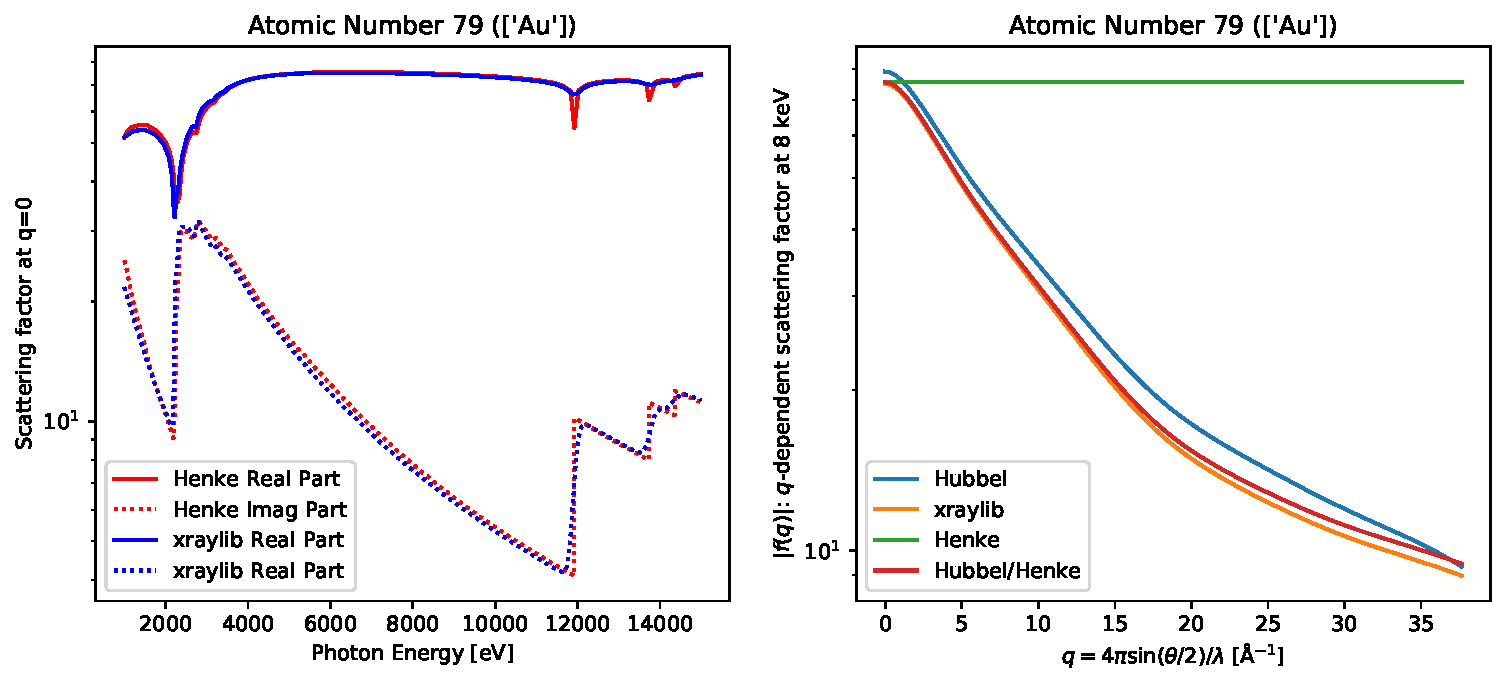
\includegraphics[width=\textwidth]{figures/formfactor_79.pdf} 
   \caption{Energy-dependent form factor in the forward scattering direction and the $Q$-dependent form factor.
   Comparison between Henke tables and \texttt{xraylib} for gold.  The plots were generated with the file
   \texttt{developer/rkirian/misc/scattering\_factors.py}.}
   \label{fig:forms}
\end{figure} 


\section{reborn}

These Henke scattering factors (at $q=0$) are returned as a single complex number $f$ from the function
\texttt{get\_scattering\_factors(Z,E)}, which is in the \texttt{reborn.target.atoms} sub-module.
\texttt{reborn} also has wrappers to the xraylib functions for convenience since they use different
units and they are not vectorized functions (hence they are very slow).  The combined Hubbel form
factors and Henke dispersion corrections may be accessed through the function
\texttt{reborn.target.atoms.hubbel\_henke\_atomic\_form\_factors}.




%%%%%%%%%%%%%%%%%%%%%%%%%%%%%%%%%%%%%%%%%%%%%%%%%%%%%%%%%%%%%%%%%%%%%%%%%
\section{From Hubbel form factors to scattering density}
%%%%%%%%%%%%%%%%%%%%%%%%%%%%%%%%%%%%%%%%%%%%%%%%%%%%%%%%%%%%%%%%%%%%%%%%%

\emph{Note: we have abandoned this approach in favor of the analytic Fourier 
transform of the Cromer-Mann expressions.}

We are provided with $f(q)$ from the Hubbel tables, along with the relation 
\begin{align}
  \rho(r) &= \frac{1}{2 \pi^2} \int_0^\infty     [q f(q)]  \frac{\sin(qr)}{r}dq  \;. \label{eqn:trans}
\end{align}
Since we cannot do an analytic integral of the Hubbel form factors as we
can do for the Cromer-Mann tables, we must do a numerical integration.
Note that we should treat the case of $r\rightarrow 0$ with care since we have have $\sin(qr)/r \rightarrow q$ in that limit.  Thus we have
a separate expression for $\rho(0)$:
\begin{align}
  \rho(0) &= \frac{1}{2 \pi^2} \int_0^\infty     [q^2 f(q)]  dq  \;. \label{eqn:trans0}
\end{align}
We aim to do this integral numerically.  We will discretize both $r$ and $q$ as follows:
\begin{align}
r_n &= n\Delta r \\
q_k &= k \Delta q
\end{align}
where $n$ and $k$ are integers.  The approximate integral is
\begin{align}
\rho(r_n) &\approx  \frac{1}{2 \pi^2 n\Delta r }\sum_{k=0}^{N-1}
[k \Delta q f(k \Delta q)]  \sin(k \Delta q n\Delta r) \Delta q \; .
\end{align}
We can do the above integral quickly if we use a Fast Fourier Transform (FFT) algorithm.  To see how this is done,
firstly note that the sin transform above is just the imaginary part of the Fourier Transform.  With some foresight, we
relate our gridpoints according to $\Delta q  = 2\pi / \Delta r N$, which gives us
\begin{align}
\rho(r_n) &\approx  \frac{1}{ \pi n\Delta r^2 }\text{Im}\left\{ \frac{1}{N}\sum_{k=0}^{N-1}
[k \Delta q f(k \Delta q)]  \exp\left(2\pi i \frac{ k  n}{N}\right) \right\} \; .
\end{align}
In numpy, the inverse FFT is defined in the following way:
\begin{align}\label{eqn:idft}
a_n = \text{FFT}^{-1}\left\{ A_k \right\}_n = \frac{1}{N}\sum_{k=0}^{N-1}A_k\exp\left(2\pi i \frac{nk}{N}\right)
\qquad n = 0,\ldots,N-1
\end{align}
If we define
\begin{align}
F_k &= k \Delta q F(k \Delta q) 
\end{align}
we arrive at the desired expression
\begin{align}\label{eqn:rhor}
\rho(n \Delta r) &\approx \frac{1}{\pi n \Delta r^2 } \text{Im} \left\{ \frac{1}{N}  \sum_{k=0}^{N-1}    F_k
\exp\left( 2\pi i \frac{nk}{ N} \right) \right\} = \frac{1}{\pi n \Delta r^2 } \text{Im}\left\{ \text{FFT}^{-1}
\left\{ F_k \right\}_n\right\} \; .
\end{align}
Equation \ref{eqn:rhor} has been tested and shown to agree in the case of the hydrogen atom, as shown in figure
\ref{fig:hydrogen} (the example script \texttt{scattering\_factors.py} that generated this plot is found in reborn).
However, there are some issues that remain at this time (1) the density near $r=0$ has a noticable error, and (2) there
are oscillatory artifacts that might be due to the truncation of $f(q)$.

\begin{figure}[htbp]
   \centering
   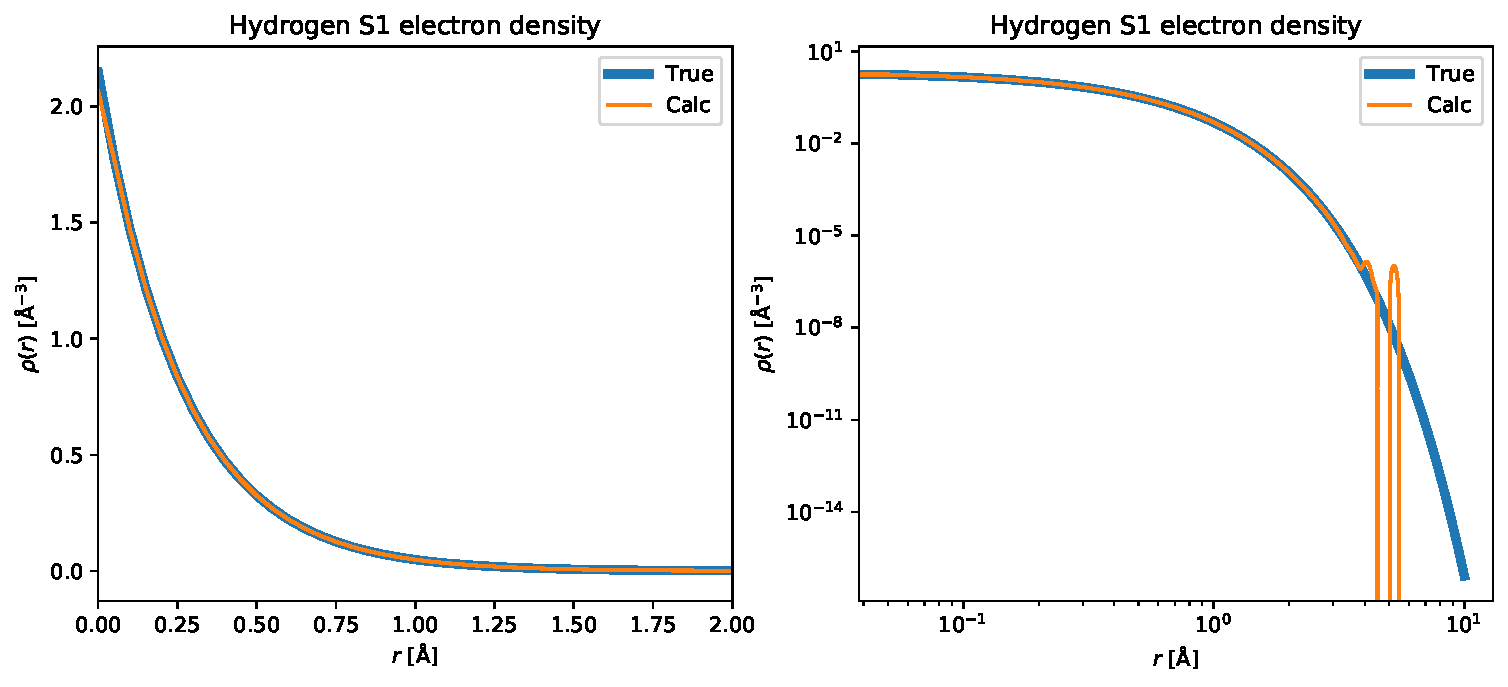
\includegraphics[width=\textwidth]{figures/hydrogen_density_1.pdf} 
   \caption{Hydrogen density calculated according to equation \ref{eqn:rhor}, compared against the analytic wavefunction
       $|\Psi(r)|^2=e^{-2 r/a_0}/\pi a_0^3$.}
   \label{fig:hydrogen}
\end{figure}

\newpage

\section{Appendix}

\subsection{Fourier transform of rotationally symmetric object}
\label{sec:3d1d}

If we consider just a single atom situated at the origin, the atomic form factor is equal to
\begin{align}
 f(\vec{q})  = \int \rho(r) \exp(-i \vec{q}\cdot\vec{r}) \; d^3r \; .
\end{align}
Due to rotational symmetry, we are free to choose a convenient direction $\vec{q} = q \hvec{z}$ such that in the
spherical coordinate system we have $\vec{q}\cdot\vec{r} =  q r \cos\theta$.  Now we write down our Fourier transform with
reference only to the magnitudes $q$ and $r$:
\begin{align}
f(\vec{q})  &= \int_0^{2\pi} d\phi \int_0^\infty \rho(r) r^2 dr \int_0^\pi \sin\theta d\theta  \exp(-i q r \cos\theta)\\
&=2\pi \int_0^\infty \rho(r) r^2 dr \int_{-1}^1  d\cos\theta  \exp(-i q r \cos\theta)  \\
&=2\pi \int_0^\infty \rho(r) r^2 dr \frac{1}{-iqr}\int_{iqr}^{-iqr}  du  \exp(u)  \\
&=2\pi \int_0^\infty \rho(r) r^2 dr \frac{\exp(iqr) - \exp(-iqr)}{iqr}   \\
f(q) &= \int_0^\infty \rho(r)   \frac{\sin(qr)}{qr}  4\pi r^2 dr  
\end{align}

\subsection{Fourier transform of hydrogen atom density}
\label{sec:hydrogenft}

\begin{align}
f_n(q)  &= \int_0^\infty \frac{1}{\pi a_0^3}e^{-2r/a_0}   \frac{\sin(qr)}{qr}  4\pi r^2 dr \\
% &= \frac{4}{q a_0^3}\int_0^\infty e^{-2r/a_0}   \sin(qr)  r dr \\
&= \frac{2}{ i q a_0^3}\int_0^\infty e^{-2r/a_0} \qty(e^{iqr} - e^{-iqr})    r dr \\
% &= -\frac{2}{q a_0^3}\pdv{q}\int_0^\infty e^{-2r/a_0} \qty(e^{iqr} + e^{-iqr})     dr \\
&= -\frac{2}{q a_0^3}\pdv{q}\int_0^\infty\qty( e^{(iq-2/a_0)r} + e^{-(iq+2/a_0)r})     dr \\
% &= \frac{2}{q a_0^3}\pdv{q} \qty( \frac{e^{(iq-2/a_0)r}}{iq-2/a_0} + \frac{e^{-(iq+2/a_0)r}}{-(iq+2/a_0)})     \eval^0_\infty \\
% &= \frac{2}{q a_0^3}\pdv{q} \qty( \frac{1}{iq-2/a_0} - \frac{1}{iq+2/a_0})     \\
% &= \frac{2}{q a_0^3}\pdv{q} \qty( \frac{-2/a_0}{q^2+4/a_0^2} - \frac{2/a_0}{q^2+4/a_0^2})     \\
&= -\frac{8}{q a_0^4}\pdv{q} \qty( \frac{1}{q^2+4/a_0^2} )     \\
&= \qty( \frac{1}{1+a_0^2q^2/4} )^2     \\
% &= -\frac{4}{q a_0^4}\pdv{q} \qty( \frac{1}{q^2-4/a_0^2} + \frac{1}{q^2+4/a_0^2})     \\
% &= -\frac{4}{q a_0^4}\pdv{q} \qty( \frac{q^2+4/a_0^2}{q^4-16/a_0^4} + \frac{q^2-4/a_0^2}{q^4-16/a_0^4})     \\
% &= -\frac{8}{q a_0^4}\pdv{q}  \frac{1}{q^2-16/q^2a_0^4}      \\
% &= -\frac{8}{q a_0^4}  \frac{1}{\qty(q^2-16/q^2a_0^4)^2}  \qty(2q+32/q^3a_0^4)    \\
% &= -\frac{16}{ q^4 a_0^4}  \frac{1}{\qty(1-16/q^4a_0^4)^2}  \qty(1+16/q^4a_0^4)    \\
\end{align}

\subsection{Fourier transform of a Gaussian}
\label{sec:gaussianft}

We wish to compute the Fourier transform of the Gaussian $g(q) = \exp(-b q^2)$:
\begin{align}
\widetilde g(r) &=  \int \exp(-b q^2) \exp(\pm i \vec q \cdot \vec r) d^3q \;.
\end{align}
This works out to the product of three integrals of the form
\begin{align}
\int_{-\infty}^\infty \exp(-b q^2 \pm i q x)dq &= \int_{-\infty}^\infty \exp\qty(-b \qty[\qty(q \pm \frac{i x}{2b} )^2 - \qty(\frac{i x}{2b})^2] )dq  \\
&= \exp\qty(-\frac{x^2}{4b})\int_{-\infty}^\infty \exp\qty(-b \qty(q \pm \frac{i x}{2b} )^2  )dq \\
&= \frac{1}{\sqrt{b}}\exp\qty(-\frac{x^2}{4b})\int_{-\infty}^\infty \exp\qty( -u^2  )du \;.
\end{align}
Finally, in doing the Gaussian integral we have
\begin{align}
\widetilde g(r) = \qty(\frac{\pi}{b})^{3/2}\exp\qty(-\frac{r^2}{4b}) \;.
\end{align}


\subsection{Gaussian integral}
\label{sec:gaussianint}

The trick is to first take the square of the 1D Gaussian integral:
\begin{align}
\int_{-\infty}^\infty \exp\qty( -u^2  )du = \qty[ \iint_{-\infty}^\infty \exp\qty( -x^2-y^2  )dxdy ]^{1/2} \;.
\end{align}
The 2D integral is then changed to polar coordinates for an easy $u$ substitution:
\begin{align}
\int_0^{2\pi} \int_0^\infty \exp\qty( -r^2  ) r dr d\phi &= \pi \int_0^\infty \exp\qty( -r^2  ) d r^2 = \pi \;.
\end{align}
Finally, the integral is equal to 
\begin{align}
 \int_{-\infty}^\infty \exp\qty( -u^2  )du = \sqrt{\pi} \;.
\end{align}

\subsection{Fourier transform of a constant}
\label{sec:ftconst}

We suspect that the Fourier transform of a constant,
\begin{align}
\int_{-\infty}^\infty \exp(iqx) dq \;,
\end{align}
is a Dirac delta function, since it is clearly infinite if $x=0$ and it seems to
be zero otherwise.  To confirm this suspicion, we take the integral
\begin{align}
\lim_{\epsilon \rightarrow 0}\int_{-\epsilon}^\epsilon \rho(x)dx &= \lim_{\epsilon \rightarrow 0}\int_{-\epsilon}^\epsilon \int_{-\infty}^\infty \exp(iqx) dq dx \\
&= \lim_{\epsilon \rightarrow 0} \int_{-\infty}^\infty \qty[ \frac{\exp(iq\epsilon)}{iq}  - \frac{\exp(-iq\epsilon)}{iq} ] dq \\
&= 2 \lim_{\epsilon \rightarrow 0} \int_{-\infty}^\infty \frac{\sin(q\epsilon)}{q} dq \\
&= 2 \int_{-\infty}^\infty \frac{\sin(q)}{q} dq \\
&= 2\pi 
\end{align}
where the last integral is that of a sinc function (section \ref{sec:sincint}).
Finally, we have our result:
\begin{align}
\frac{1}{2\pi}\int_{-\infty}^\infty \exp(iqx) dq = \delta(x) \;.
\end{align}


\subsection{Integral of a sinc function}
\label{sec:sincint}

We can cheat a little bit, since we know the sinc function is the Fourier 
transform of a tophat, and we know that the zero-frequency term of a Fourier
transform is the integral of the function.  This is what we want to prove:
\begin{align}
 \int_{-\infty}^\infty \frac{\sin(q)}{q} dq = \pi
\end{align}
Start by taking the Fourier transform of a tophat function of width $2L$:
\begin{align}
 \int_{-L}^{L} \exp(iqx) dx = \frac{\exp(iqx)}{iq}\eval_{-L}^{L} = 2 \frac{\sin(qL)}{q} \;.
\end{align}
Now do the inverse Fourier transform
\begin{align}
\frac{1}{2\pi}\int_{-\infty}^{\infty} 2 \frac{\sin(qL)}{q} \exp(-iqx) dx = 1 \; \text{if} \; -L < x < L \;.
\end{align}
Taking the zero frequency ($x=0$) value we have
\begin{align}
\int_{-\infty}^{\infty} \frac{\sin(q)}{q} dq = \pi \;.
\end{align}

\newpage

\bibliography{\jobname}
\bibliographystyle{plain}

\end{document}
